\section{XLABEL Plot X-axis Label Function}

\subsection{Usage}

This command adds a label to the x-axis of the plot.  The general syntax
for its use is
\begin{verbatim}
  xlabel('label')
\end{verbatim}
or in the alternate form
\begin{verbatim}
  xlabel 'label'
\end{verbatim}
or simply
\begin{verbatim}
  xlabel label
\end{verbatim}
Here \verb|label| is a string variable.  You can also specify properties
for that label using the syntax
\begin{verbatim}
  xlabel('label',properties...) 
\end{verbatim}
\subsection{Example}

Here is an example of a simple plot with a label on the \verb|x|-axis.
@>
which results in the following plot.


\centerline{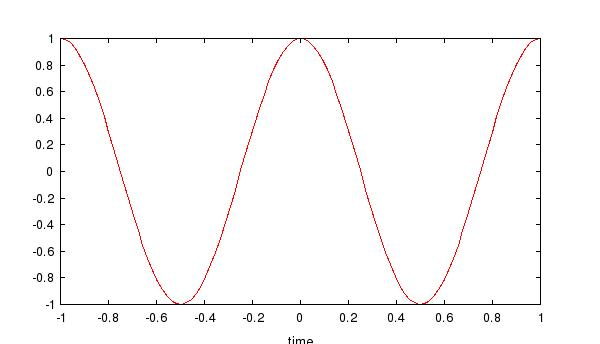
\includegraphics[width=8cm]{xlabel1}}

